\section{Exceptional Control Flow}

\begin{concept}{Exception Types}\\
Two main categories of exceptions:

\textbf{Interrupt Sources:}
\begin{itemize}
  \item Peripherals requesting immediate CPU attention
  \item Software-generated interrupts
  \item Asynchronous to instruction execution
\end{itemize}

\textbf{System Exceptions:}
\begin{itemize}
  \item \textbf{Reset}: Processor restart
  \item \textbf{NMI}: Non-maskable Interrupt (cannot be ignored)
  \item \textbf{Faults}: Undefined instructions, errors
  \item \textbf{System Calls}: OS services (SVC and PendSV)
\end{itemize}
\end{concept}

\begin{definition}{Interrupt Control}\\
PRIMASK register controls interrupt handling:
\begin{itemize}
  \item Single bit controls all maskable interrupts
  \item Reset state: PRIMASK = 0 (interrupts enabled)
  \item Control methods:
    \begin{itemize}
      \item Assembly: \texttt{CPSID i} (disable), \texttt{CPSIE i} (enable)
      \item C: \texttt{\_\_disable\_irq()}, \texttt{\_\_enable\_irq()}
    \end{itemize}
\end{itemize}

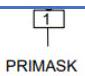
\includegraphics[width=\linewidth]{images/2024_12_29_79e6b22f503fb7b4f718g-11}
\end{definition}

\begin{definition}{Context Storage}\\
Interrupt handling requires automatic context saving:

\textbf{ISR Entry:}
\begin{itemize}
  \item Stores on stack:
    \begin{itemize}
      \item xPSR, PC, LR, R12
      \item R0-R3 (caller-saved registers)
    \end{itemize}
  \item Stores EXC\_RETURN in LR
\end{itemize}

\textbf{ISR Exit:}
\begin{itemize}
  \item Via BX LR or POP {..., PC}
  \item Restores from stack:
    \begin{itemize}
      \item R0-R3, R12, LR, PC
      \item xPSR
    \end{itemize}
\end{itemize}
\end{definition}

\begin{concept}{Polling vs Interrupts}\\
\textbf{Polling Approach:}
\begin{itemize}
  \item Periodic status register checks
  \item Synchronous with main program
  \item \textbf{Advantages:}
    \begin{itemize}
      \item Simple implementation
      \item Predictable timing
      \item No extra hardware needed
    \end{itemize}
  \item \textbf{Disadvantages:}
    \begin{itemize}
      \item CPU wastes time waiting
      \item Reduced system throughput
      \item Longer response times
    \end{itemize}
\end{itemize}

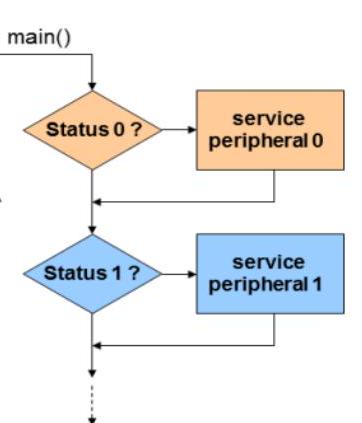
\includegraphics[width=\linewidth]{images/2024_12_29_79e6b22f503fb7b4f718g-11(1)}

\textbf{Interrupt Approach:}
\begin{itemize}
  \item Hardware-triggered event handling
  \item Asynchronous to main program
  \item \textbf{Advantages:}
    \begin{itemize}
      \item Efficient CPU usage
      \item Quick response times
      \item Better system throughput
    \end{itemize}
  \item \textbf{Disadvantages:}
    \begin{itemize}
      \item More complex implementation
      \item Harder to debug
      \item Timing less predictable
    \end{itemize}
\end{itemize}

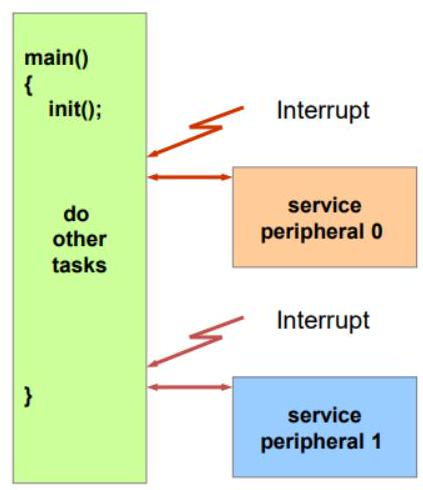
\includegraphics[width=\linewidth]{images/2024_12_29_79e6b22f503fb7b4f718g-11(2)}
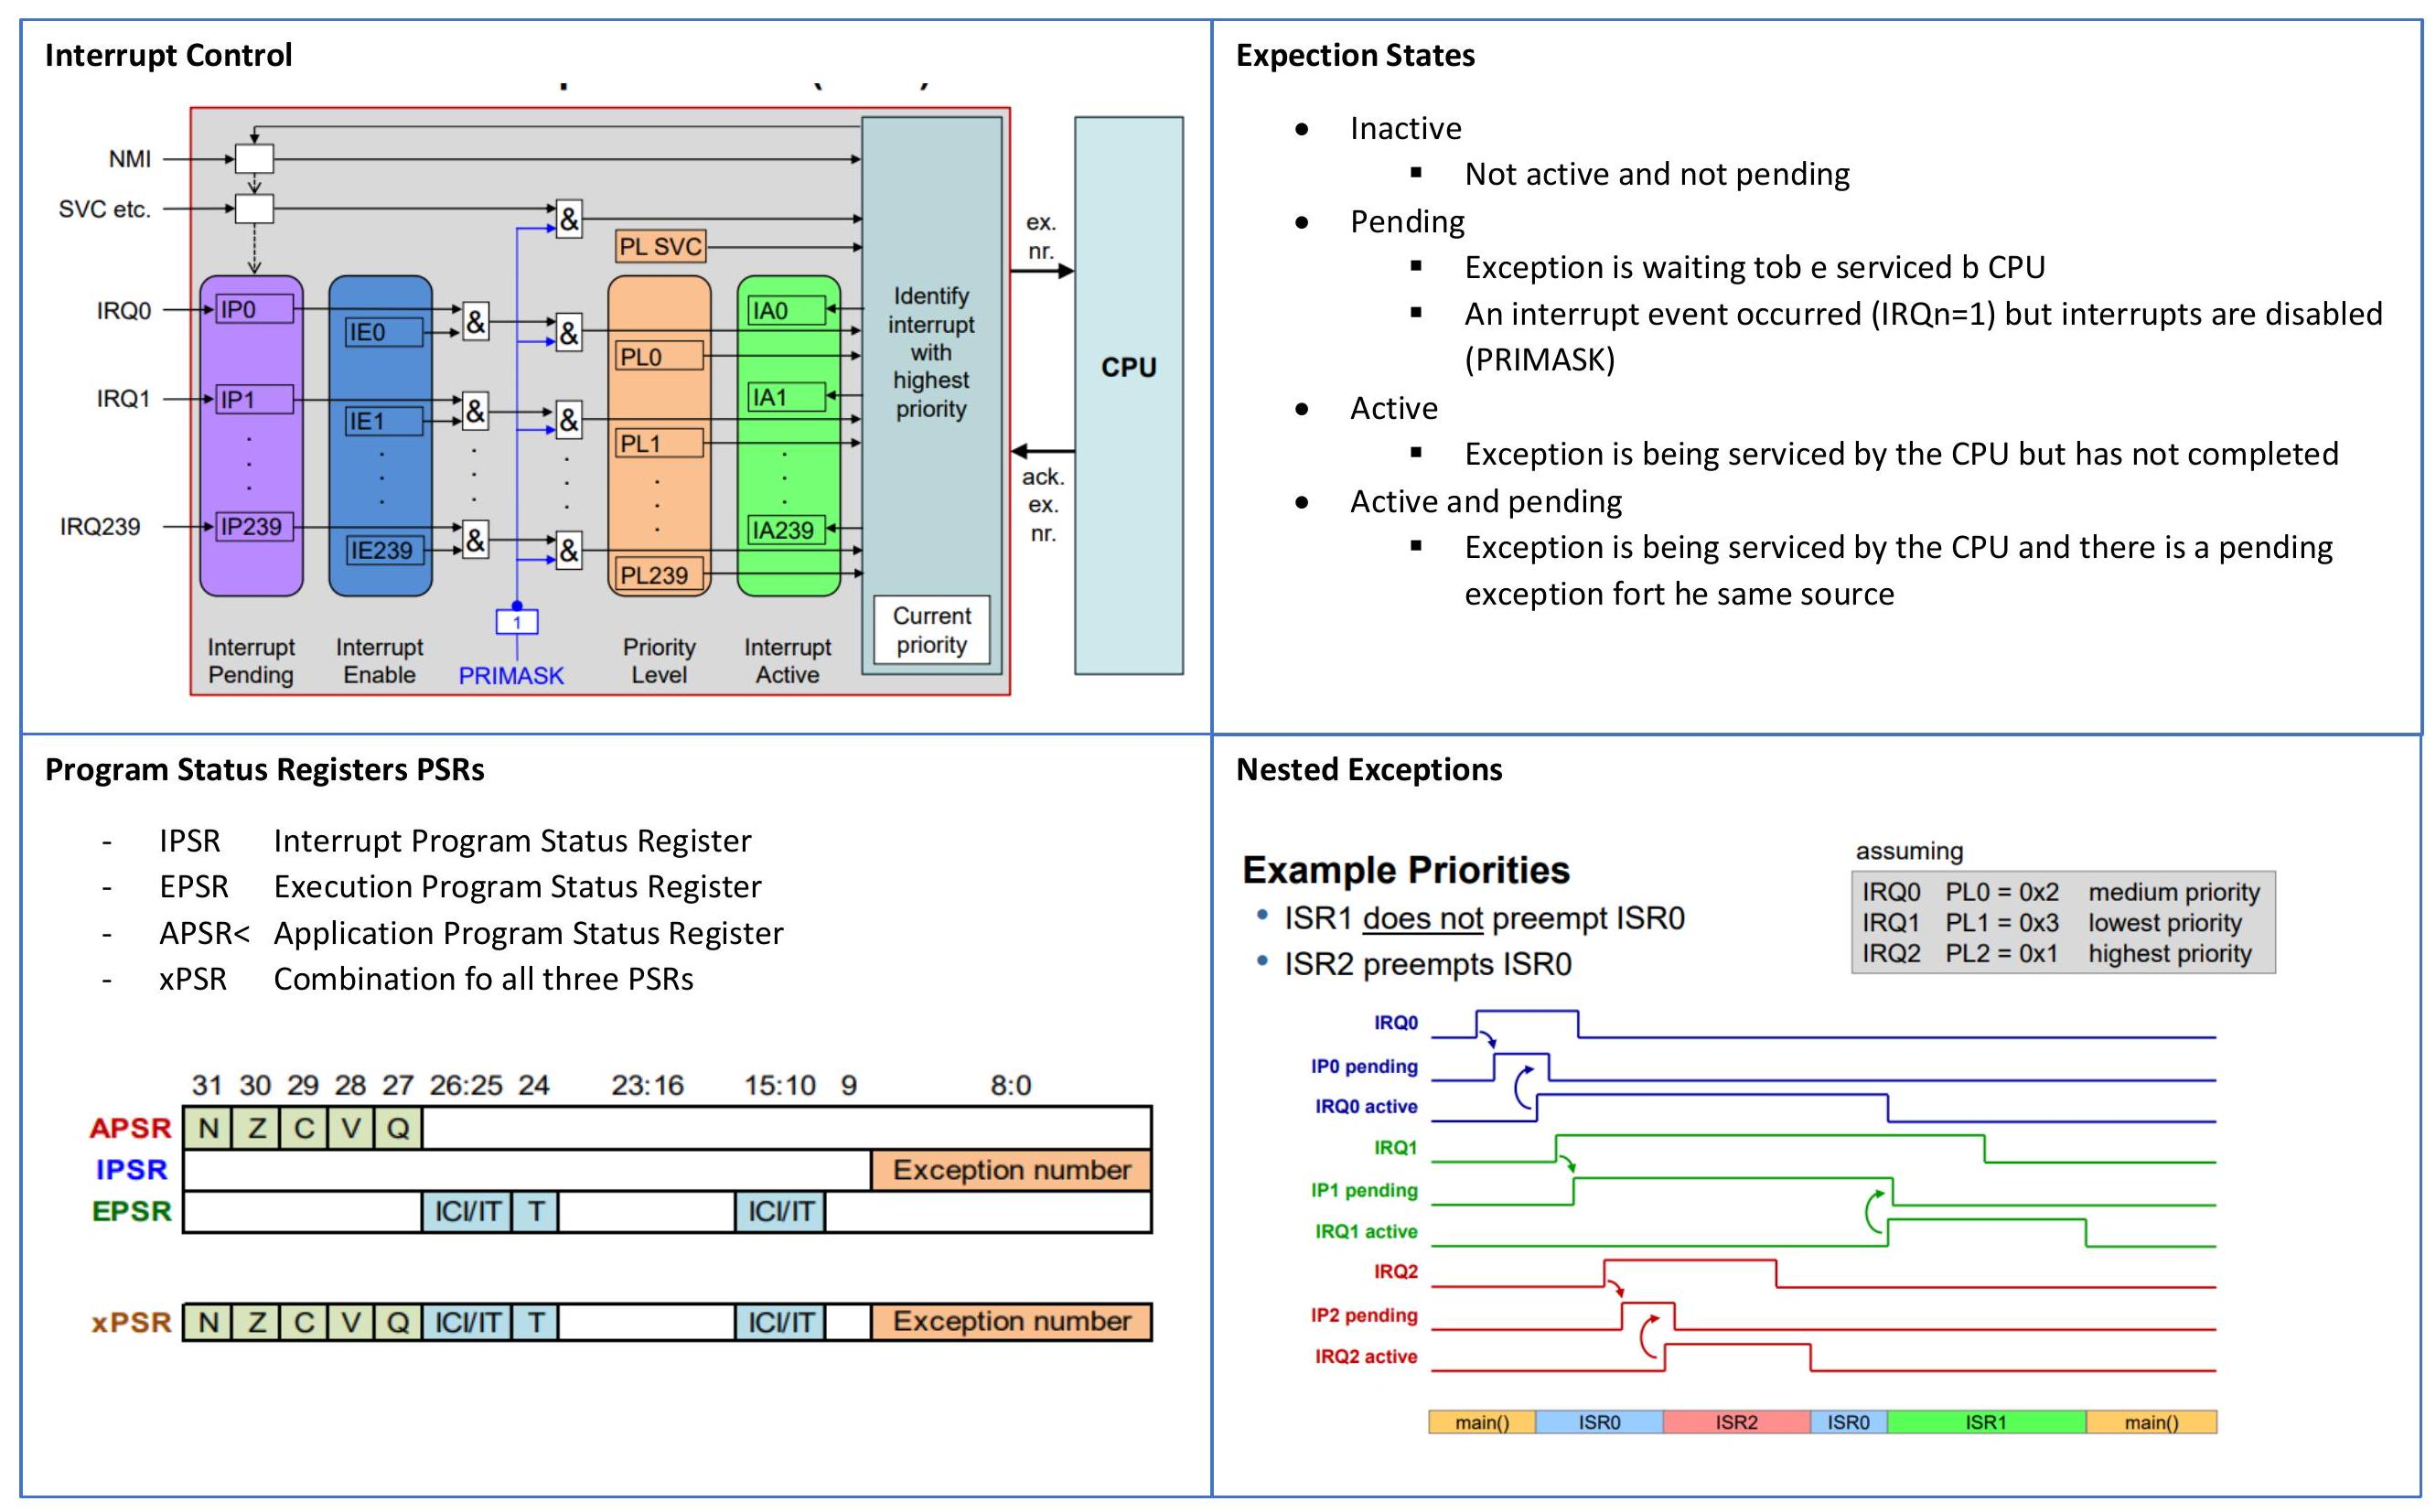
\includegraphics[width=\linewidth]{images/2024_12_29_79e6b22f503fb7b4f718g-12}
\end{concept}

\begin{example2}{Basic ISR Implementation}
\begin{lstlisting}[language=armasm, style=basesmol]
    ; Interrupt Service Routine
    EXPORT MyISR
MyISR
    PUSH    {R4-R7, LR}    ; Save registers
    
    ; Handle interrupt here
    ; R0-R3 already saved automatically
    
    POP     {R4-R7, PC}    ; Restore and return
\end{lstlisting}
\end{example2}

\begin{KR}{Implementing Interrupt Handlers}\\
Steps for implementing interrupt handlers:
\begin{enumerate}
  \item Define interrupt vector
  \item Save necessary context
  \item Handle the interrupt
  \item Clear interrupt flag
  \item Restore context
  \item Return from interrupt
\end{enumerate}

Important considerations:
\begin{itemize}
  \item Keep ISRs short
  \item Handle critical tasks only
  \item Be aware of nested interrupts
  \item Protect shared resources
\end{itemize}
\end{KR}